\documentclass{beamer}
\usepackage[T1]{fontenc}
\usepackage[english]{babel}
\usefonttheme{serif}
\setbeamertemplate{navigation symbols}{
\usebeamerfont{footline}
\usebeamercolor[fg]{footline}
\insertframenumber/\inserttotalframenumber{}
}
\setbeamerfont{frametitle}{size = \small}
\usepackage{mathpazo}
\usepackage{float}
\usepackage[labelsep = colon]{caption}
\usepackage{amsmath}
\usepackage{setspace}
\usepackage{graphicx}
\usepackage{threeparttablex}
\usepackage{longtable}
\usepackage{booktabs}
\usepackage{dcolumn}
\usepackage{pdfpages}


\title{GV217 Conflict Analysis}
\subtitle{Week 18: Terrorism}
\author{Muzhou Zhang\\ muzhou.zhang@essex.ac.uk\\ Virtual Office Hour: 15:30--16:30, Friday, 997 5800 8679}
\date{04 Feb 2022}

\begin{document}
\maketitle
\setstretch{1.25}

\begin{frame}{Elements of Terrorism}
    \begin{itemize}
        \pause\item Non-state actors
        \pause\item Political or social goals
        \pause\item Civilian or non-combatant targets 
        \pause\item Violence
        \pause\item Intimidating wide audience
    \end{itemize}
\end{frame}

\begin{frame}{Trend of Terrorism}
    \pause
    \begin{center}
        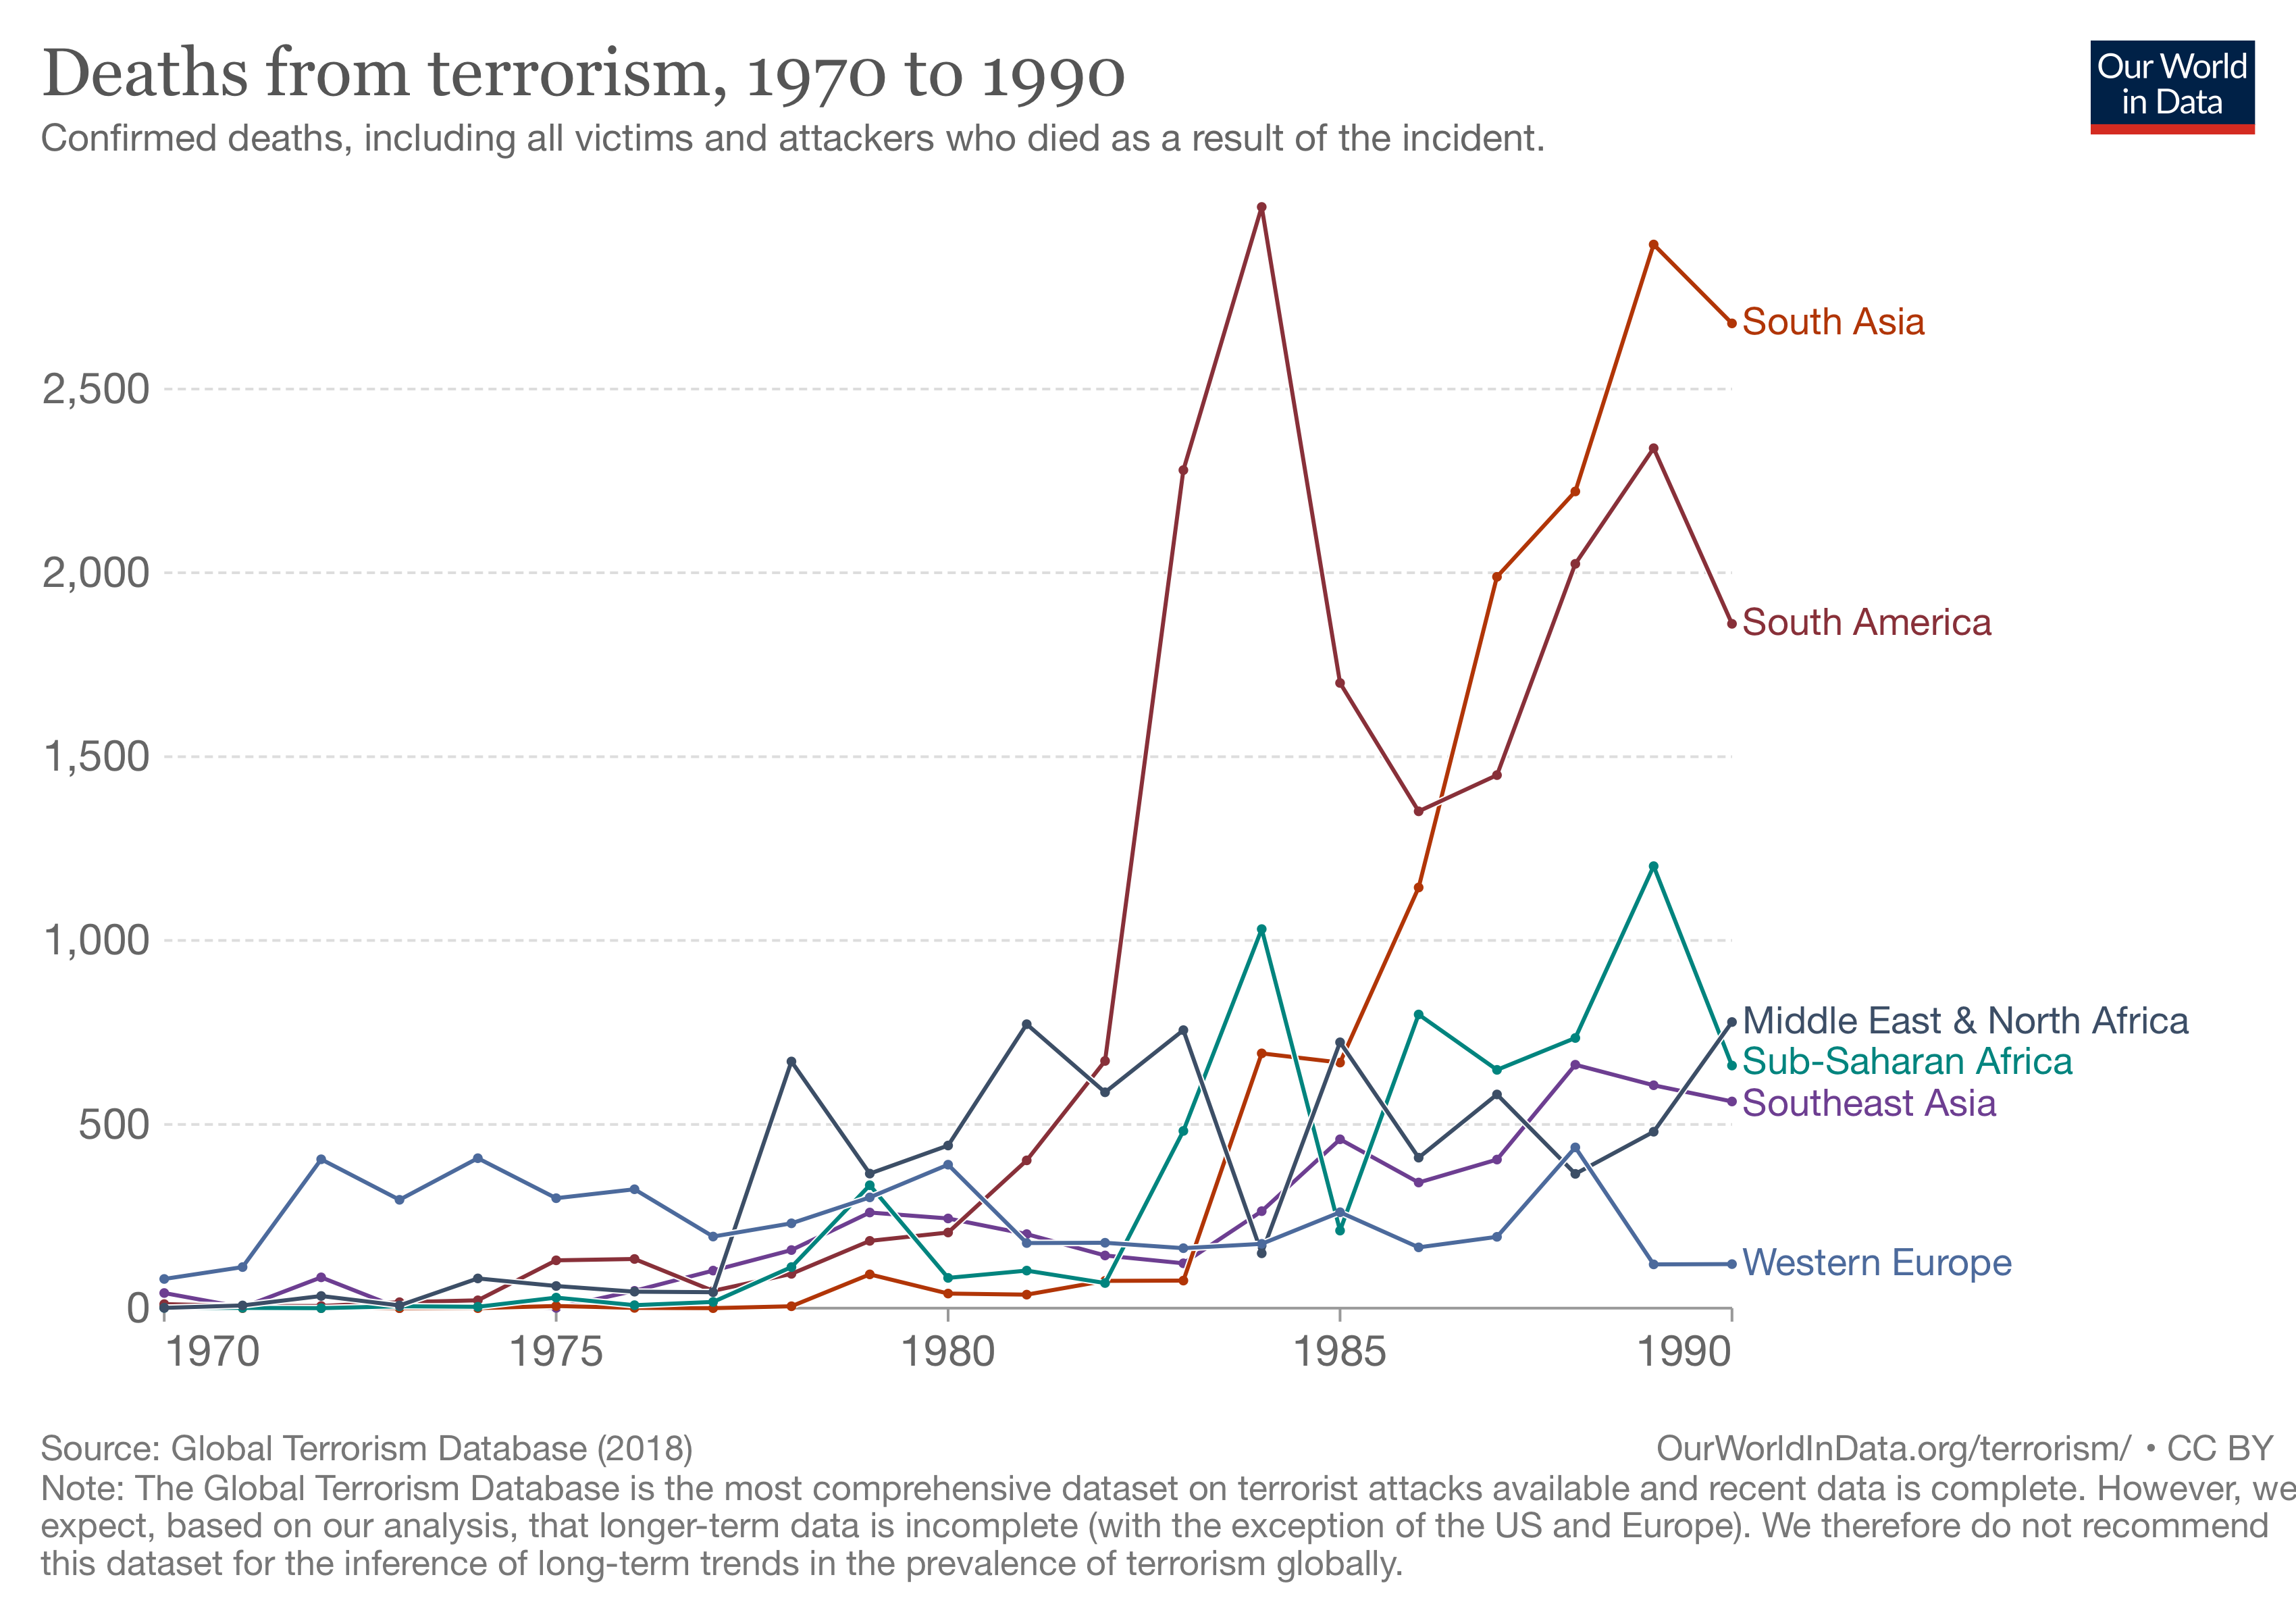
\includegraphics[width = \linewidth]{/Users/mz/Desktop/GitHub/teaching/gv217_conflict_analysis/figs/wk18/terrorism_1990.png}
    \end{center}
\end{frame}

\begin{frame}{Trend of Terrorism}
    \pause
    \begin{center}
        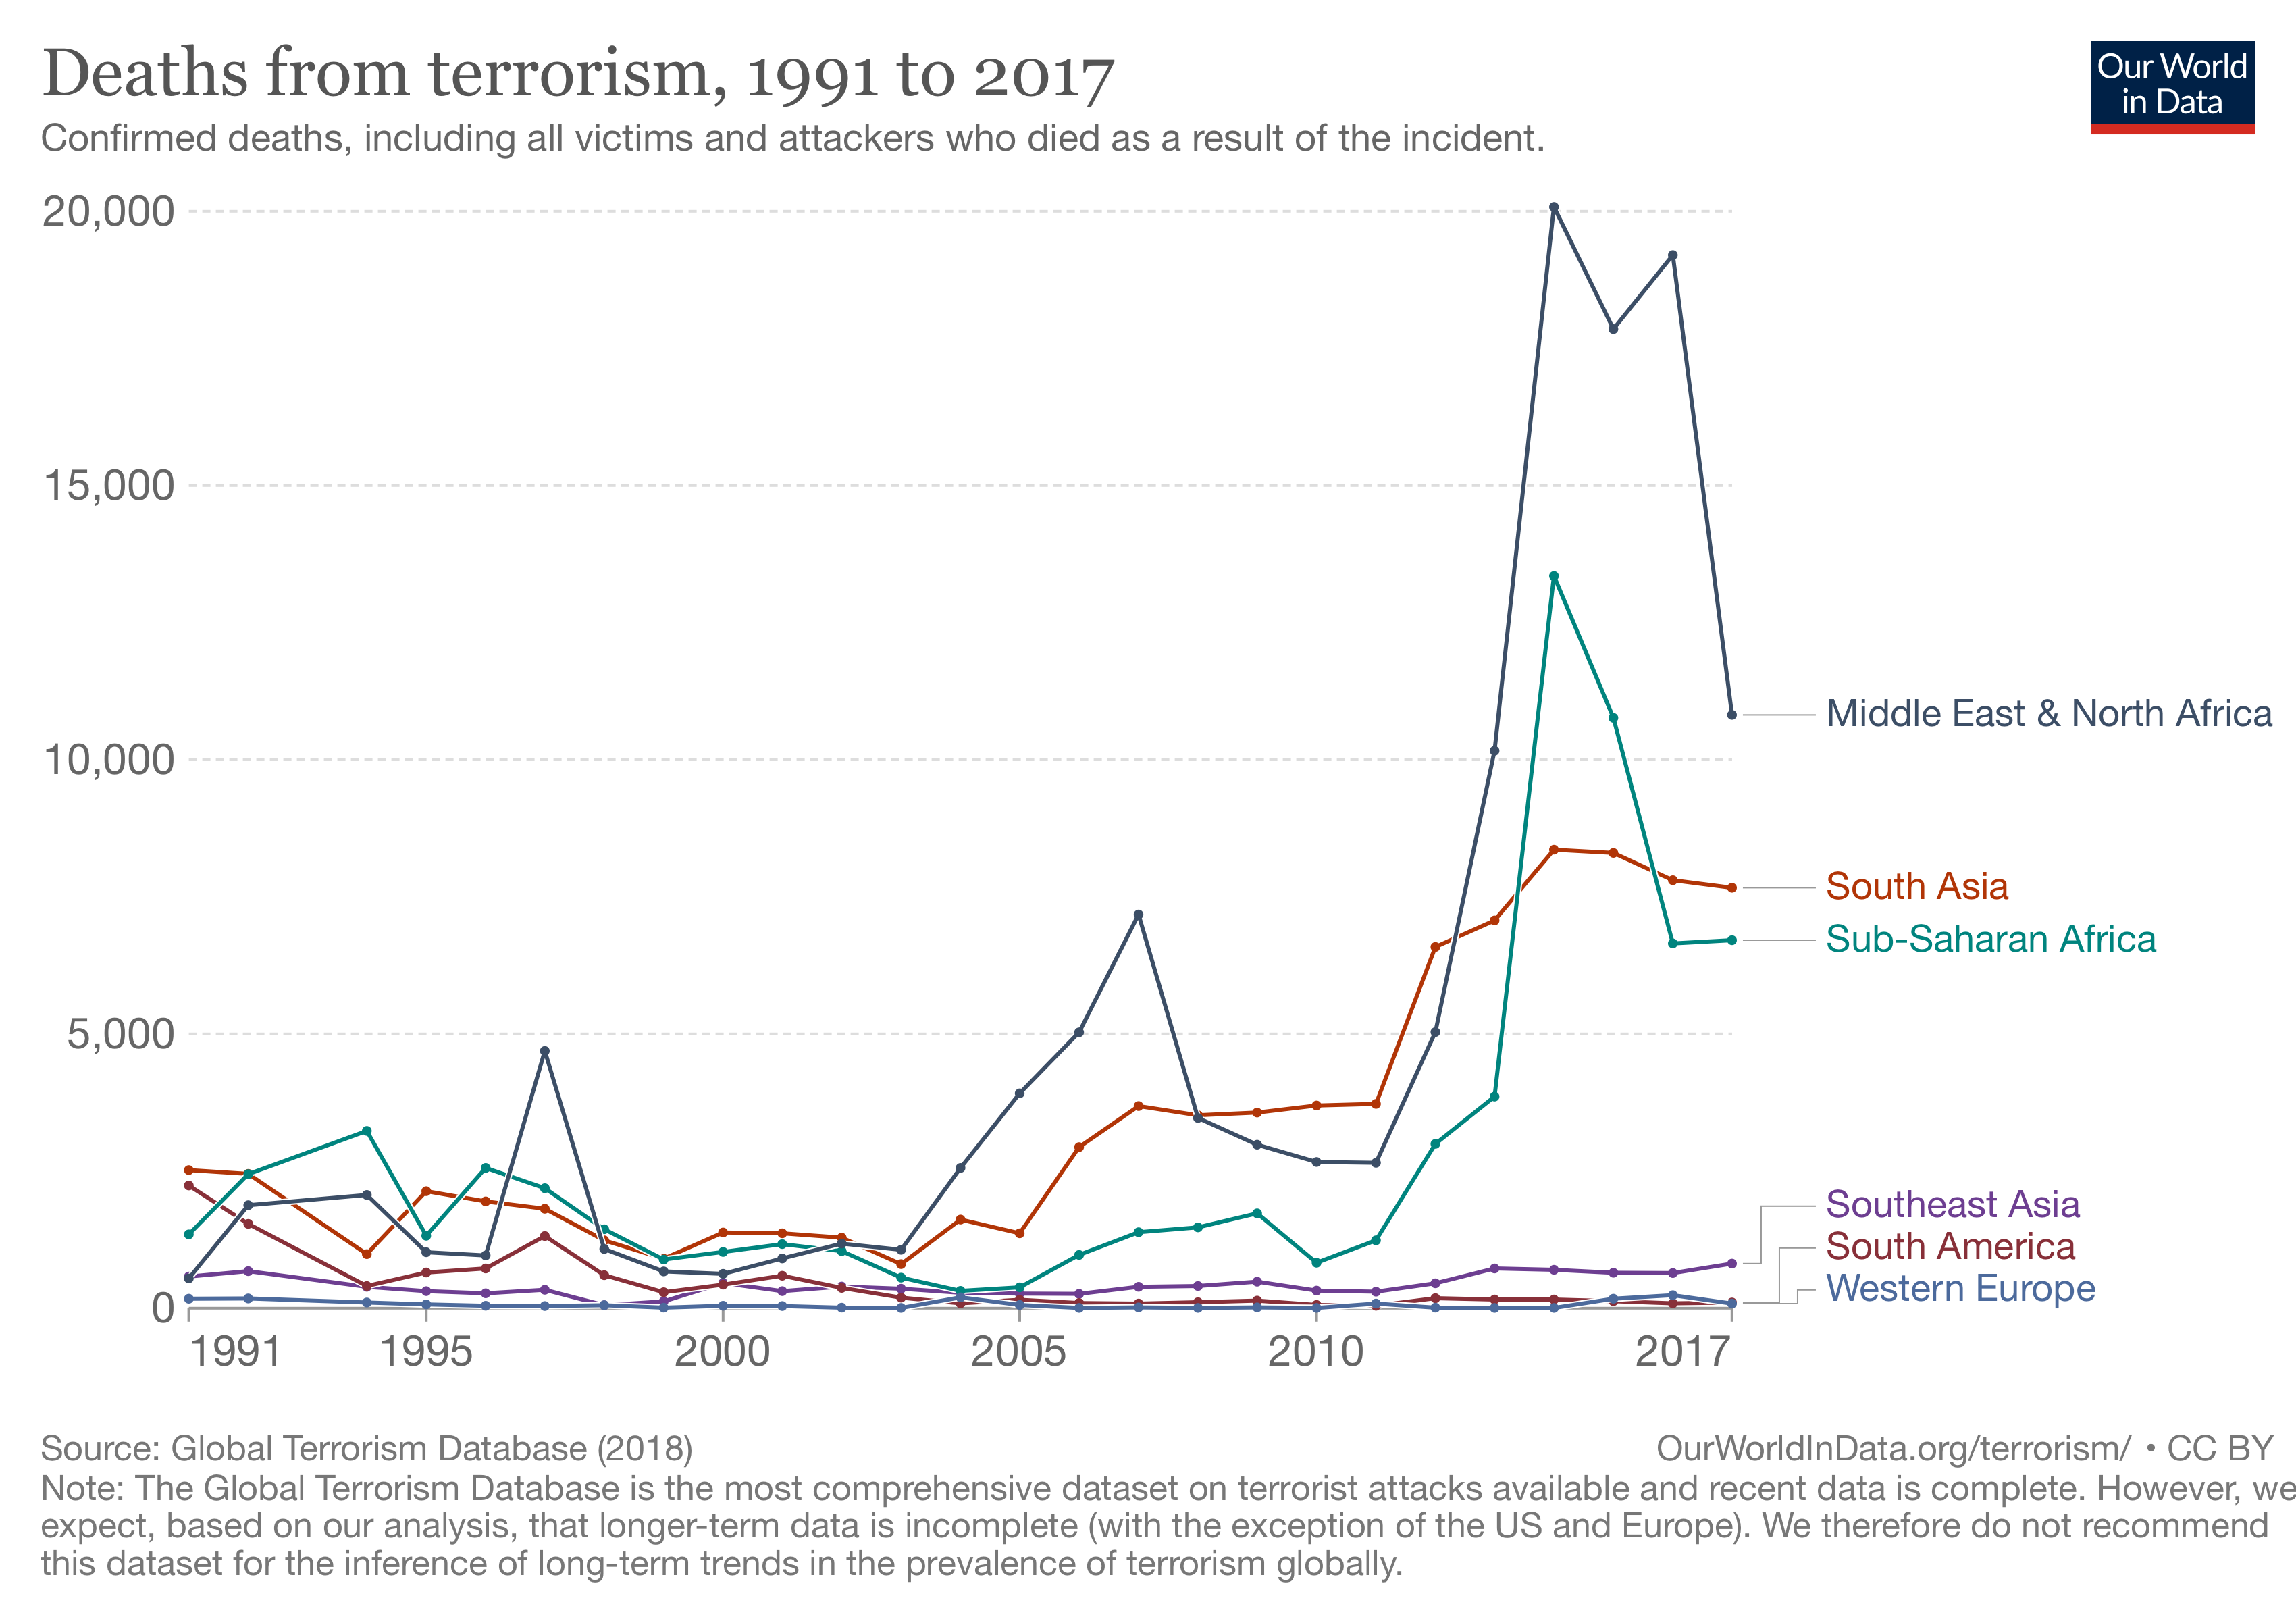
\includegraphics[width = \linewidth]{/Users/mz/Desktop/GitHub/teaching/gv217_conflict_analysis/figs/wk18/terrorism_2017.png}
    \end{center}
\end{frame}

\begin{frame}{Trend of Terrorism}
    \pause
    \begin{center}
        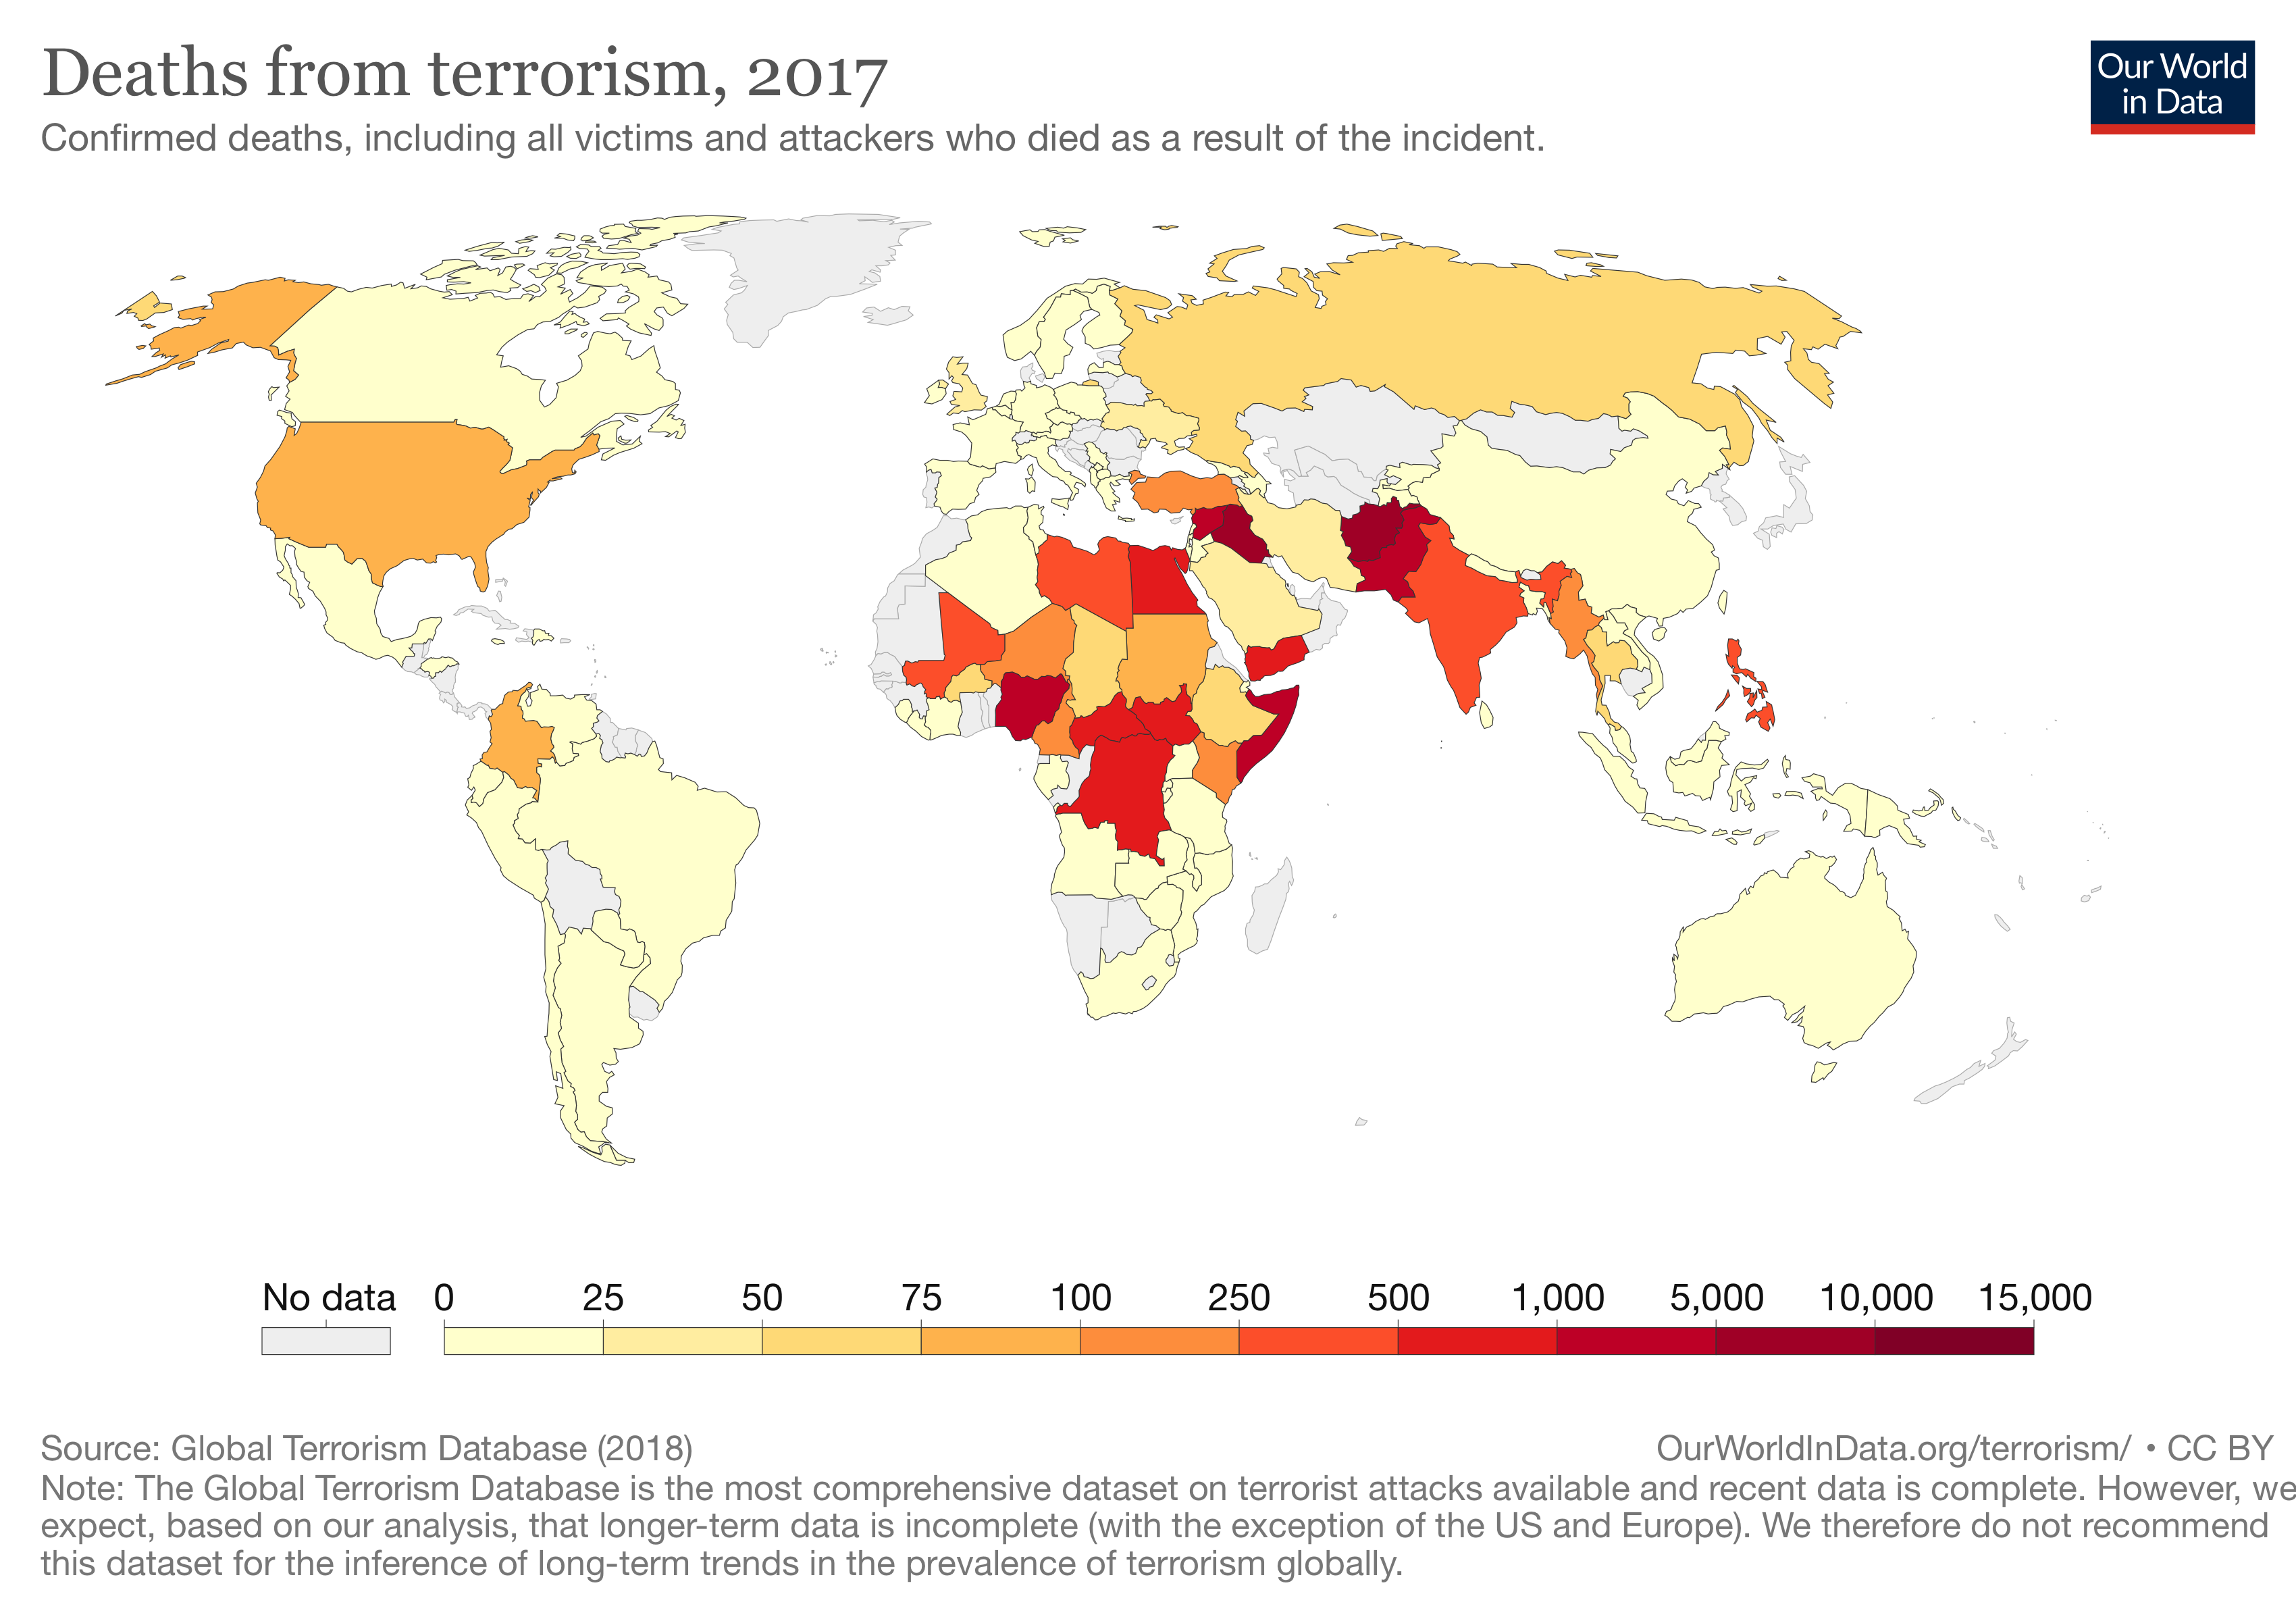
\includegraphics[width = \linewidth]{/Users/mz/Desktop/GitHub/teaching/gv217_conflict_analysis/figs/wk18/terrorism_2017_map.png}
    \end{center}
\end{frame}

\begin{frame}{Designation of Terrorist Organizations}
    \pause
    Foreign Terrorist Organization (FTO) Designation Process
    \begin{center}
        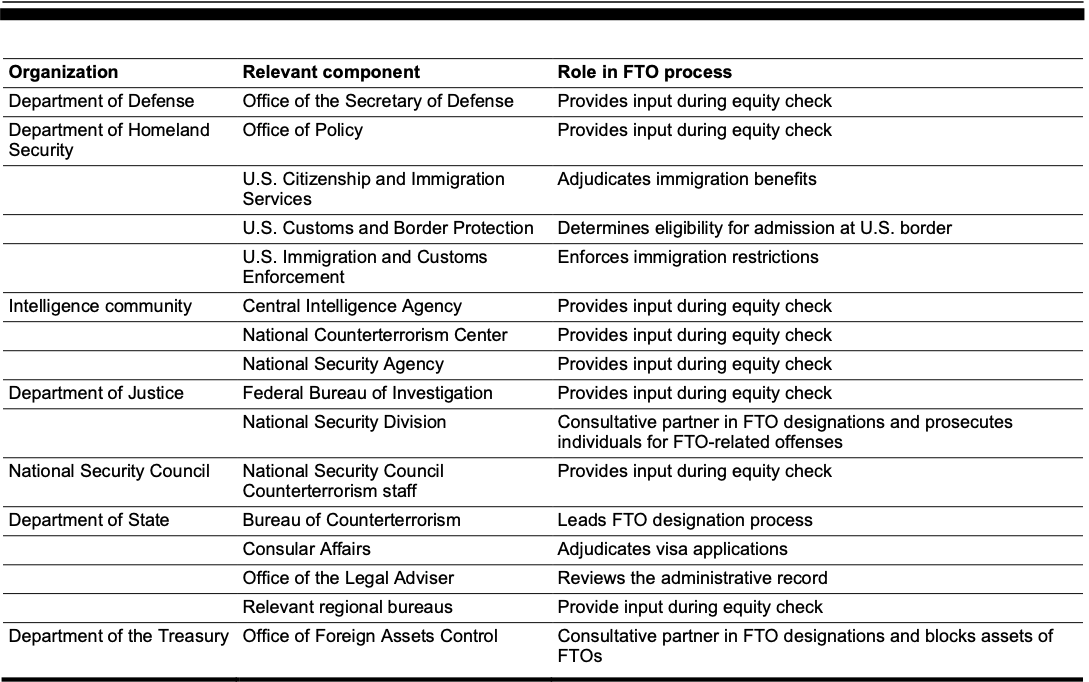
\includegraphics[width = \linewidth]{/Users/mz/Desktop/GitHub/teaching/gv217_conflict_analysis/figs/wk18/us_designation.png}
    \end{center}
    \footnotesize Source: Appendix II, GAO-15-629
\end{frame}

\begin{frame}{Designation of Terrorist Organizations}
    \pause
    \begin{center}
        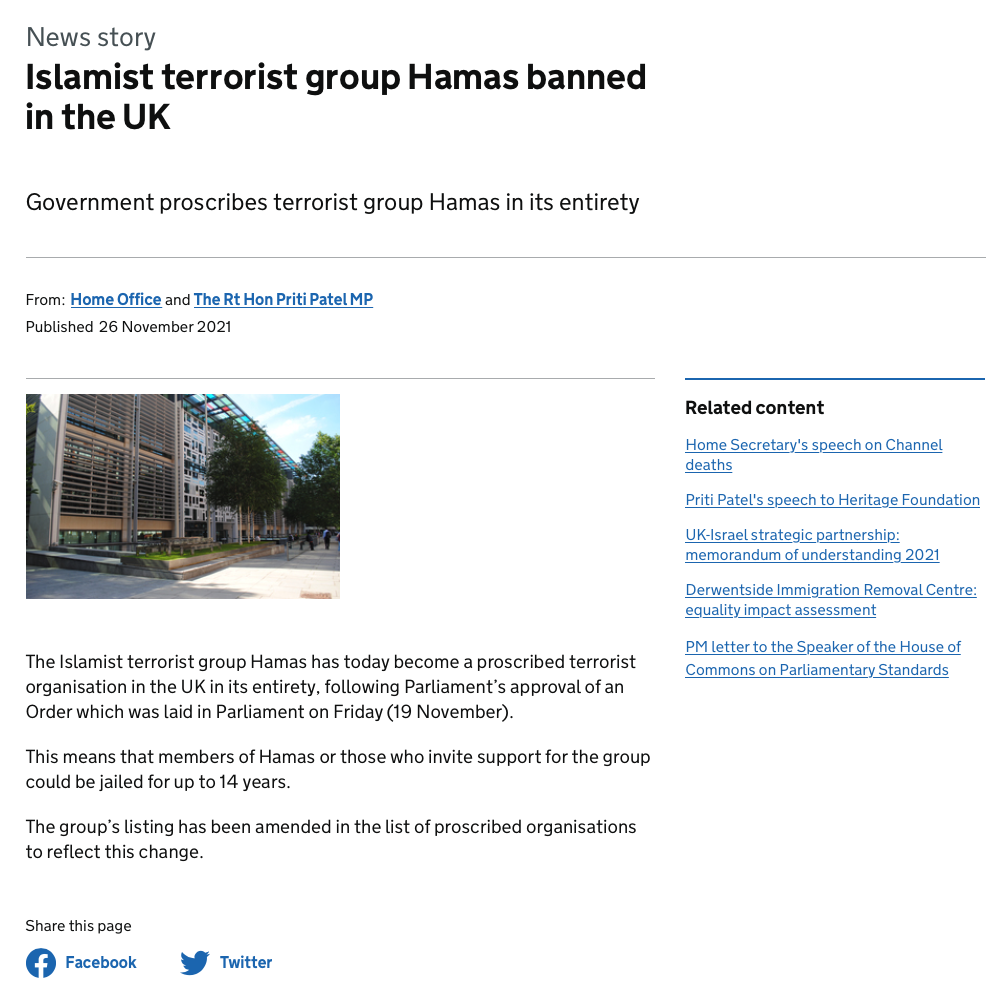
\includegraphics[height = 0.60\linewidth]{/Users/mz/Desktop/GitHub/teaching/gv217_conflict_analysis/figs/wk18/hamas_uk.png}
    \end{center}
    \footnotesize Source: https://www.gov.uk/government/news/islamist-terrorist-group-hamas-banned-in-the-uk
\end{frame}

\begin{frame}{Designation of Terrorist Organizations}
    \pause
    Five Eyes Designation Lists (Selected)
    \begin{center}
        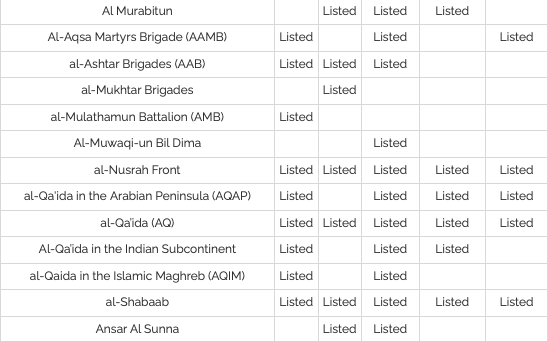
\includegraphics[height = 0.50\linewidth]{/Users/mz/Desktop/GitHub/teaching/gv217_conflict_analysis/figs/wk18/five_eyes.png}
    \end{center}
    \footnotesize Source: https://www.terroristdesignations.org/five-eyes/
\end{frame}

\begin{frame}{Designation of Terrorist Organizations}
    \pause
    Designation of Ethnic Terrorist Groups, 1970--2016 (\(N = 127\))
    \begin{center}
        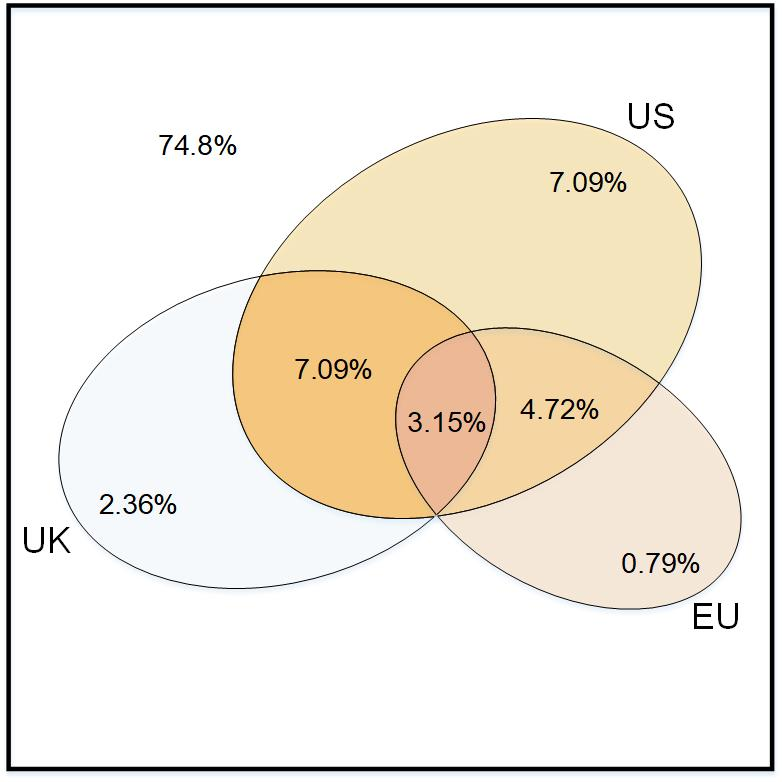
\includegraphics[height = 0.50\linewidth]{/Users/mz/Desktop/GitHub/teaching/gv217_conflict_analysis/figs/wk18/jeyabraba_phillips.png}
    \end{center}
    \footnotesize Source: Jeyabraba \& Phillips
\end{frame}

\begin{frame}{Who Uses Terrorism? How?}
\framesubtitle{Polo \& Gleditsch (2016)}
    \begin{itemize}
        \pause\item Militarily weaker rebels carry out a larger number of attacks
        \pause\item Rebels w/ universal ideologies, and thus, larger audience, are more likely to attack hard/official targets
\end{itemize}
\end{frame}

\begin{frame}{Who Uses Terrorism? How?}
\framesubtitle{Polo \& Gleditsch (2016)}
    \pause
    \begin{center}
        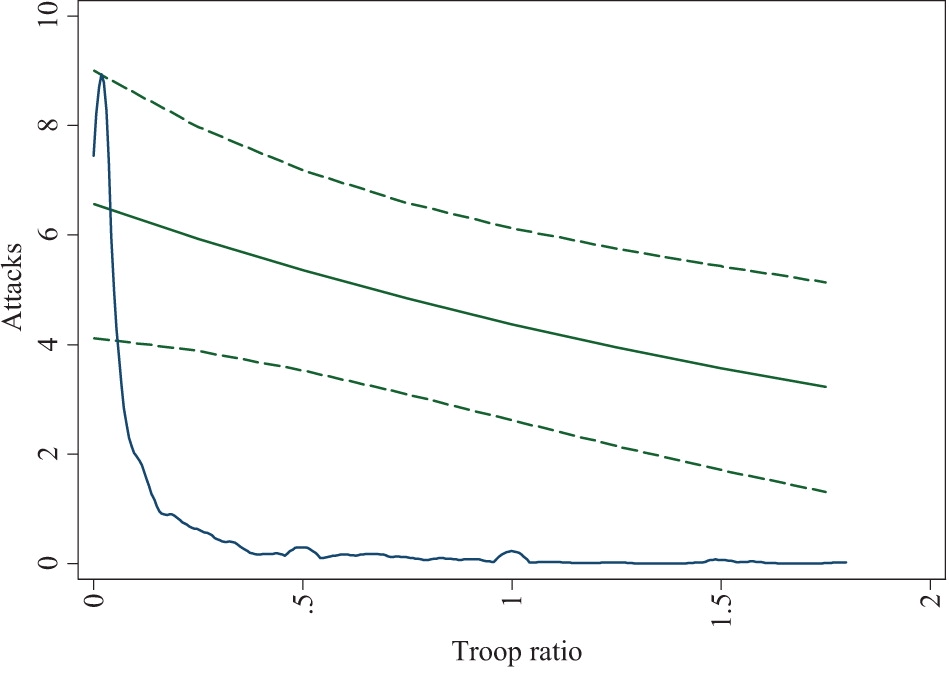
\includegraphics[height = 0.60\linewidth]{/Users/mz/Desktop/GitHub/teaching/gv217_conflict_analysis/figs/wk18/polo_gleditsch_fig3.png}
    \end{center}
    \footnotesize Source: Figure 3 (upper panel)
\end{frame}

\begin{frame}{Who Uses Terrorism? How?}
\framesubtitle{Polo \& Gleditsch (2016)}
    \pause
    \begin{center}
        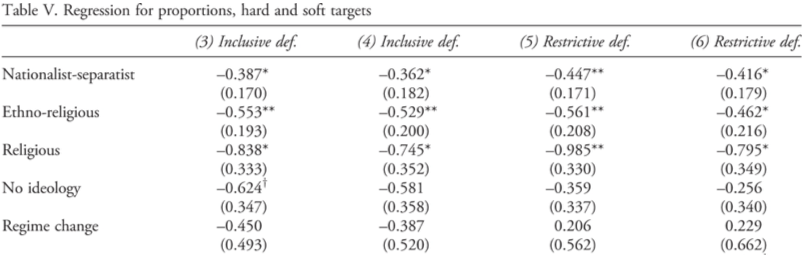
\includegraphics[height = 0.50\linewidth, width = \linewidth]{/Users/mz/Desktop/GitHub/teaching/gv217_conflict_analysis/figs/wk18/polo_gleditsch_tab5.png}
    \end{center}
    \footnotesize Source: Table 5
\end{frame}

\begin{frame}{Is Terrorism Effective?}
\framesubtitle{Fortna (2015)}
    \pause
    \begin{center}
        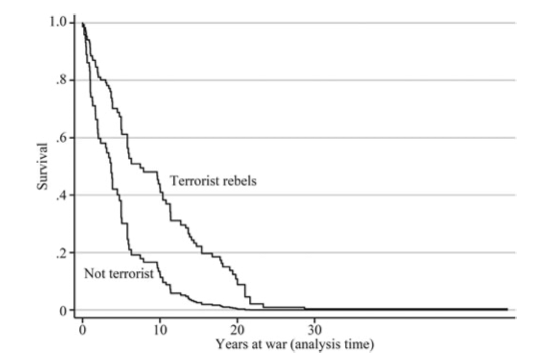
\includegraphics[height = 0.60\linewidth]{/Users/mz/Desktop/GitHub/teaching/gv217_conflict_analysis/figs/wk18/fortna_fig5.png}
    \end{center}
    \footnotesize Source: Figure 5
\end{frame}

\begin{frame}{Is Terrorism Effective?}
\framesubtitle{Fortna (2015)}
    \pause
    \begin{center}
        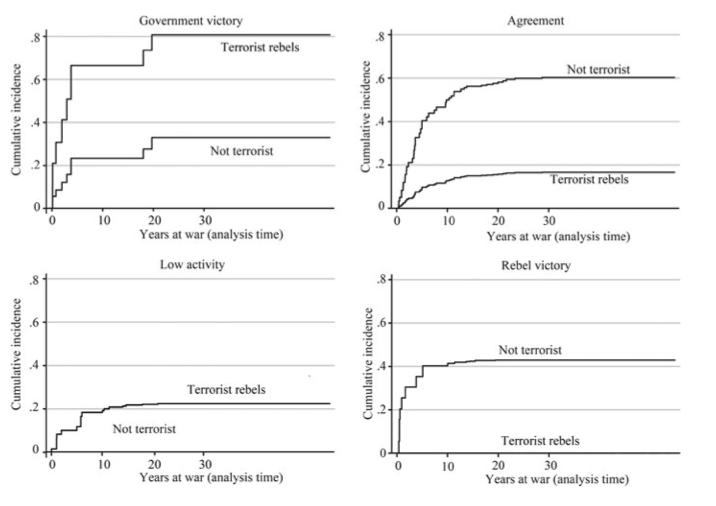
\includegraphics[height = 0.60\linewidth]{/Users/mz/Desktop/GitHub/teaching/gv217_conflict_analysis/figs/wk18/fortna_fig6.png}
    \end{center}
    \footnotesize Source: Figure 6
\end{frame}

\begin{frame}{Is Terrorism Effective?}
\framesubtitle{Fortna (2015)}
    \begin{itemize}
        \pause\item Wars involving terrorist rebels are likely to last longer
        \pause\item Terrorist rebels are less likely than nonterrorist rebels to achieve military victory or settlements
    \end{itemize}
\end{frame}

\begin{frame}{Is Terrorism Effective?}
\framesubtitle{Thomas (2014)}
    \pause
    \begin{center}
        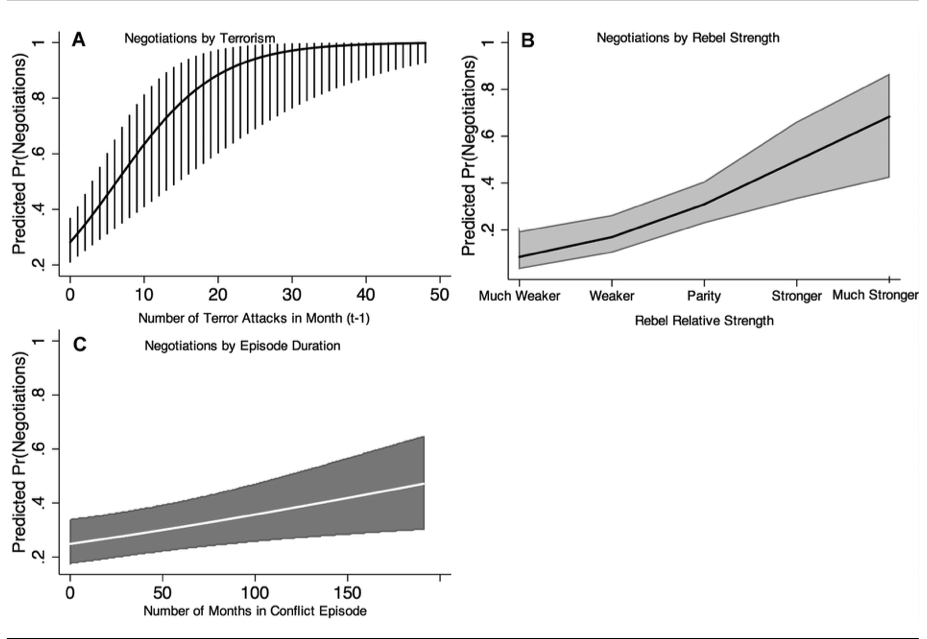
\includegraphics[height = 0.60\linewidth]{/Users/mz/Desktop/GitHub/teaching/gv217_conflict_analysis/figs/wk18/thomas_fig2.png}
    \end{center}
    \footnotesize Source: Figure 2
\end{frame}

\begin{frame}{More Research Questions}
    \begin{itemize}
        \pause\item Are carrots or sticks more effective in deterring terrorism? What's the scope condition? (Asal, Brian, Rethemeyer et al. 2019)
        \pause\item Under what circumstances rebel groups are more likely to resort to terrorist attacks? (Polo \& González 2020)
        \pause\item Why terrorist attacks occur more frequently in certain areas within a country? (Welsh forthcoming)
    \end{itemize}
\end{frame}

\end{document}
